\documentclass[11pt]{article}
\usepackage[utf8]{inputenc}
\usepackage[T1]{fontenc}
\usepackage[francais]{babel}
\usepackage[francais]{layout}
\usepackage{hyperref}
\selectlanguage{french}

% NE PAS CHANGER !!
\ifx \public \undefined \def\public{etudiants} \fi
\usepackage[\public]{tps}
\usepackage{tikz}

% Numéro du TP
\newcommand{\numtd}{03}
% Titre du TP
\newcommand{\titretd}{Construire un vrai ordinateur ?}
\def\tup#1{\langle #1\rangle}
\begin{document}

\entete{\numtd}{\titretd}

\section{Introduction}

Dans ce TP, on va essayer de construire un petit ordinateur à partir d'une porte \texttt{NAND} seulement. Pour ce faire on va construire des unités logiques de plus en plus compliquées jusqu'à avoir un ordinateur capable de faire tourner des programmes. Pour ce TP, on va utiliser un Hardware Simulator. Son rôle sera de vérifier que vos unités logiques (\textit{chips}) sont bien implémentées. De plus, il vous aidera aussi pour vos déboguer vos chips.

Le langage dans lequel vous allez écrire vos chips est un DSL (Domain Specific Language). C'est à dire que c'est un langage spécifiquement dédié à l'écriture de vos chips. Dans la prochaine section, je vais brièvement décrire ce langage afin que vous puissiez écrire rapidement vos premiers chips. N'hésitez-pas à me poser des questions sur le langage, notamment lorsque vous écrirez des chips utilisant des bus de données.

Chaque chip vient en trois fichiers :
\begin{itemize}
\item \texttt{XXX.hdl} : c'est dans ce fichier que vous écrirez le code de vos chips
\item \texttt{XXX.tst} : ce fichier est déjà écrit pour vous et contient des tests.
\item \texttt{XXX.cmp} : ce fichier est aussi déjà écrit et contient la sortie des tests.
\end{itemize}

Les deux derniers fichiers sont utilisés par le Hardware Simulator pour vérifier la correction de vos chips. A priori, vous éditerez seulement les fichiers dont l'extension est \texttt{.hdl}.

\subsection*{Utilisation du Hardware Simulator} Une fois le Hardware Simulator lancé, pour vérifier votre chip vous devez faire deux étapes :
\begin{itemize}
\item Cliquer sur le bouton \textbf{load chip} pour charger le fichier \texttt{.hdl}
\item Cliquer sur le bouton \textbf{load script} pour charger le fichier \texttt{.tst}
\item Enfin, cliquer sur le bouton \textbf{run} (double flèche bleue) pour lancer les tests
\end{itemize}

Pour gagner du temps, je vous invite à sélectionner l'option \textbf{no animation} dans le menu \textbf{animation}.
\subsection*{Plan}

Ce TP est découpé en \(4\) sections :
\begin{enumerate}
\item Dans la section~\ref{sec:base}, vous implémenterez les chips de base : \texttt{And}, \texttt{Or}, ...
\item Dans la section~\ref{sec:alu}, on s'intéressera à la conception d'un ALU (Arithmetic Logic Unit)
\item Dans la section~\ref{sec:memory}, on s'intéressera à des chips non-séquentiels afin de créer la mémoire (RAM) de notre ordinateur
\item Dans la section~\ref{sec:computer}, on réunira les différents CHIPS écrits dans les sections précédentes pour fabriquer l'ordinateur.
\end{enumerate}

L'archive contenant le projet est trouvable ici : \url{https://www.lsv.fr/~fthire/teaching/2018-2019/archisys/TP/3/bootstrap.tar.gz}.
\section{Hardware Language}

Le \textit{Hardware Language} est un langage qui permet de programmer les chips. Tous les chips que vous allez écrire respectent le format suivant (exemple de la porte \texttt{AND}) :
\begin{verbatim}
/**
 * And gate:
 * out = 1 if (a == 1 and b == 1)
 *       0 otherwise
 */

CHIP And {
    IN a, b;
    OUT out;

    PARTS:
    //TODO
}
\end{verbatim}

Chaque chip commence par un commentaire résumant le comportement attendu du chip. Ensuite, le code d'un chip se découpe en trois parties :
\begin{itemize}
\item \textit{IN} : cette ligne donne des noms aux pins d'entrée. Ici, la porte \texttt{AND} à deux pins en entrée nommés \texttt{a} et \texttt{b}
\item \textit{OUT} : cette ligne donne des noms aux pins de sortie. Ici, la porte \texttt{AND} à un seul pin de sortie nommé \texttt{out}
\item \textit{PART} : Cette partie contient le programme que vous allez écrire pour implémenter le chips. Cette partie est composées d'une suite d'\texttt{instruction} (décrit ci-dessous) séparés par des points-virgules.
\end{itemize}

Le format d'une instruction est le suivant :
\begin{verbatim}
XXX(ipin1=var1, ipin2=var2, ..., opin1=var3, opin2=var4, ...)
\end{verbatim}

La sémantique de cette instruction est qu'elle appelle le chip \texttt{XXX} :
\begin{itemize}
\item elle branche sur le pin d'entrée \texttt{ipin1} le pin \texttt{var1}, sur le pin d'entrée \texttt{ipin2} le pin \texttt{var2}.
\item \texttt{var3} est le nouveau nom du pin de sortie \texttt{opin1}, et \texttt{var4} est le nouveau nom du pin de sortie \texttt{opin2}
\end{itemize}

Pour les deux premières sections, il est attendus que \texttt{var3} et \texttt{var4} soient des nouveaux noms (de nouvelles variables sont créees), tandis que \texttt{var1} et \texttt{var2} sont des noms qui doit déjà exister.

Par exemple, lorsque vous voulez créer un nouveau chip et vous souhaitez utiliser le chip \texttt{AND}, vous pouvez écrire l'instruction suivante :
\begin{verbatim}
...
AND(a=a1,b=a2, out=outand)
\end{verbatim}

en supposant que les variables \texttt{a1} et \texttt{a2} existent déjà.

\section{Les chips de base}
\label{sec:base}
On suppose dans cette partie que le chip \texttt{NAND} est déjà construit. Son interface est la suivante :
\begin{verbatim}
/**
 * Nand gate:
 * out = 1 if (a == 0 and b == 0)
 *       0 otherwise
 */

CHIP Nand {
    IN a, b;
    OUT out;

    PARTS:
    BUILTIN
}
\end{verbatim}

C'est le seul chip que vous pourrez utiliser au début. Une fois que aurez implémenté correctement un chip, il sera utilisable pour l'implémentation des futurs chips bien entendu. Les commentaires au début de chaque fichier sont assez explicites et donc je ne rajouterai pas de commentaire. Cependant, je vous conseille d'implémenter vos chips dans l'ordre suivant :
\begin{enumerate}
\item \texttt{Not} (1 instruction)
\item \texttt{And} (2 instructions)
\item \texttt{Or} (3 instructions)
\item \texttt{Or8Way} (7 instructions)
\item \texttt{Xor} (5 instructions)
\item \texttt{Not16} (16 instructions)
\item \texttt{And16}
\item \texttt{Or16}
\item \texttt{Mux} (4 instructions)
\item \texttt{Mux16} (16 instructions)
\item \texttt{Mux4Way16} (3 instructions)
\item \texttt{Mux8Way16} (3 instructions)
\item \texttt{DMux} (3 instructions)
\item \texttt{DMux4Way} (3 instructions)
\item \texttt{DMux8Way} (5 instructions)
\end{enumerate}

\section{ALU}
\label{sec:alu}

\subsection*{Additionneur}
À partir des briques de base que l'on a construites à la section précédente, on va essayer de construire une unité d'arithmétique logique (ALU). Notre unité d'arithmétique va être capable d'additionner deux entiers binaires codés sur 16 bits, mais pas seulement. Il pourrait incrémenter/décrémenter, faire des opérations bit à bit comme \texttt{x \& y} ou \texttt{x | y}. Pour cela, un premier objectif va être de recoder une additionneur sur 16 bits. Pour cela, vous allez devoir implémenter les trois chips suivants:

\begin{enumerate}
\item \texttt{HalfAdder} (2 instructions)
\item \texttt{FullAdder} (3 instructions)
\item \texttt{Add16} (16 instructions)
\item (bonus) \texttt{Inc16} (1 instruction)
\end{enumerate}

\subsection*{ALU}

Une fois ces portes implémentées, on va s'intéresser à l'ALU. L'idée de ce chip est de prendre deux vecteurs codés sur 16 bits en entrées \(x\) et \(y\) et de calculer en sortie un vecteur de 16 bits \(out(x,y)\). \(out\) étant une fonction qui est paramétré par \(6\) flags:
\begin{itemize}
\item \(zx\), met le vecteur \(x\) à \(0\)
\item \(nx\), inverse bit à bit le vecteur \(x\)
\item \(zy\), met le vecteur \(y\) à \(0\)
\item \(ny\), inverse bit à bit le vecteur \(y\)
\item \(f\), si à \(1\) calcule la somme des deux entrées, sinon fait un \(ET\) logique bit à bit
\item \(no\), inverse bit à bit l'output
\end{itemize}

\paragraph{Préliminaires :} quelques questions avant de vous lancer dans l'implémentation (l'ordre des flags est celui présenté ci-dessus) :
\begin{itemize}
\item Quelle est la fonction \(out(x,y)\) quand on lui passe comme flag le vecteur \((0,1,0,1,0,1)\) ?
\item Quelle est la fonction \(out(x,y)\) quand on lui passe comme flag le vecteur \((0,0,1,1,0,1)\) ?
\item Quelle est la fonction \(out(x,y)\) quand on lui passe comme flag le vecteur \((1,1,1,1,1,1)\) ?
\item Est-il possible de calculer \(x+1\) ?
\item Est-il possible de calculer \(x-1\) ?
\item Est-il possible de calculer \(x-y\) ?
\end{itemize}

\paragraph{Output flag :} de plus, il vous est demandé de produire deux autres sorties :

\begin{itemize}
\item \(zr\), est à \(1\) si \(out(x,y) = 0\), \(0\) sinon
\item \(ng\), est à \(1\) si \(out(x,y) < 0\), \(0\) sinon
\end{itemize}

\paragraph{Implémentation :} maintenant, implémentez le chip suivant :
\begin{enumerate}
\item \texttt{ALU} (13 instructions)
\end{enumerate}

\section{Memory}
\label{sec:memory}

Cette partie s'intéresse à des portes logiques dont le comportement dépend du temps. Autrement dit, un des pins de sortie peut se brancher sur un des pins d'entrées. Cela implique qu'en pratique, ce style de chip utilise une horloge, qui va réguler le signal électrique. Cependant, dans notre cas, et pour simplifier le design de nos chips, on ne va pas manipuler l'horloge directement. Au lieu de ça, on va considérer qu'on a un chip \textit{built-in}, comme la porte \texttt{nand} qui nous est donné. Ce chip, appelé \texttt{DFF} recopie son entrée sur sa sortie à chaque \textit{tick} d'horloge (voir Fig.~\ref{fig:dff}). À noter qu'utiliser une horloge revient à \textit{discrétiser} le temps.

\begin{figure}
  \centering
  \label{fig:dff}
  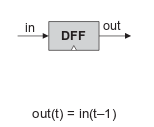
\includegraphics{pictures/dff.png}
  \caption{DFF}
\end{figure}

Pour cette partie, je vous invite à programmer vos chips dans l'ordre suivant :

\begin{enumerate}
\item \texttt{Bit} (2 instructions)
\item \texttt{Register} (16 instructions)
\item \texttt{PC} (5 instructions)
\item \texttt{RAM8} (10 instructions)
\item \texttt{RAM64} (10 instructions)
\item \texttt{RAM512} (10 instructions)
\item \texttt{RAM4K} (10 instructions)
\item \texttt{RAM16K} (6 instructions)
\end{enumerate}

\section{Assembleur}
\label{sec:assembly}

Les instructions de notre ordinateur se codent sur 16 bits. Cette partie vous donne des informations sur le fonctionnement du CPU afin de savoir comment interpréter ces instructions. Le CPU utilise trois registres : \texttt{A}, \texttt{D} et \texttt{M}. Le registre \texttt{A} peut servir à référencer des endroits de la mémoire. Il a donc une instruction dédiée afin de lui passé des adresses de 15 bits présentée en Fig.~\ref{fig:A}. Le CPU gère un deuxième type d'instruction présentée en Fig.~\ref{fig:C}. Cette instruction va passer deux registres à l'ALU, détermine quelle opération de l'ALU est demandée et affecte le résultat à un ou plusieurs registres. De plus, cette instruction peut changer le \textit{program counter} si on souhaite \textit{jumper} vers une adresse du programme. Pratique pour coder un \textbf{if ... then ... else} ou bien un boucle \textbf{while}. Pour cette instruction, le registre \texttt{D} est toujours branché au bus \(x\) de l'ALU. Le bit \(a\) de l'instruction permet de dire si le bus \(y\) sera branché au registre \texttt{A} (\(a=1\)) ou bien au registre \texttt{M} sinon. Les bits \(c1,\dots,c6\) correspondent aux flags de l'ALU. Ils sont dans le même ordre que celui donné section~\ref{sec:alu}. Les trois bits \(d1,d2,d3\) indiquent quelles registres recevront le résultat de l'ALU: \(d1\) pour le registre \texttt{A}, \(d2\) pour le registre \texttt{D} et enfin \(d3\) pour le registre \texttt{M}. Enfin, les trois \(j1,j2,j3\) indiquent s'il faut modifier la valeur du \textit{program counter} avec la valeur du registre \texttt{A}. Les différents cas sont résumés en Fig.~\ref{fig:jump}

\begin{figure}
  \centering
  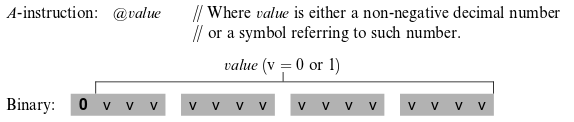
\includegraphics[scale=0.5]{pictures/instructionA.png}
  \caption{A-instruction}
  \label{fig:A}
\end{figure}

\begin{figure}
  \centering
  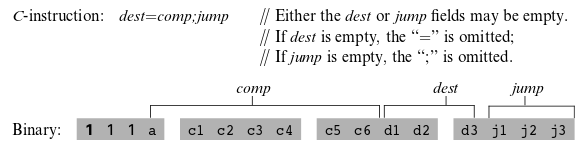
\includegraphics[scale=0.5]{pictures/instructionC.png}
  \caption{A-instruction}
  \label{fig:C}
\end{figure}

\begin{figure}
  \centering
  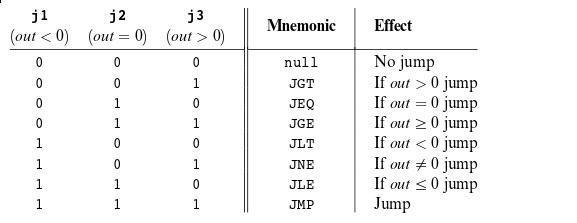
\includegraphics[scale=0.5]{pictures/jump.png}
  \caption{jump}
  \label{fig:jump}
\end{figure}

\section{Computer}
\label{sec:computer}

Dans cette partie, on va réutiliser la RAM construite à la partie précédente ainsi que notre ALU pour construire un \textit{vrai} ordinateur. Notre ordinateur va utiliser deux périphériques externes : un clavier et un écran dont la spécification vous est donnée respectivement en Fig.~\ref{fig:keyboard} et Fig.~\ref{fig:screen}. À noter que le Hardware Simulator gère les entrées/sorties pour vous. Dans notre cas, on ne s'occupera pas des entrées. Dans le Hardware Simulator, sous l'option \textbf{View} vous pouvez sélectionner \textbf{Screen} pour regarder ce que produisent certains tests (comme \texttt{ComputerRect-external.tst}). De plus, dans notre architecture, il faut charger notre programme en mémoire qui sera différent de la \texttt{RAM}. Ici, ce sera la \texttt{ROM}. Pour cela, on va aussi utiliser un chip \textit{built-in} qui simulera ce composant voir Fig.~\ref{fig:rom}. Je vous conseille d'implémenter les chips dans l'ordre suivant :

\begin{enumerate}
\item \texttt{Memory} (7 instructions)
\item \texttt{CPU} (20 instructions)
\item \texttt{Computer} (3 instructions)
\end{enumerate}

Afin de vous aider, vous trouverez en Fig.~\ref{fig:cpu}, un schéma qui résume le comportement interne du CPU.
\begin{figure}
  \centering
\begin{verbatim}
Chip Name:
Keyboard    // Memory map of the physical keyboard.
            // Outputs the code of the currently
            // pressed key.
Output:
out[16]     // The ASCII code of the pressed key, or
            // one of the special codes
Function:
Outputs the code of the key presently pressed on the
physical keyboard.
Comment:
This chip is continuously being refreshed from a
physical keyboard unit (simulators must simulate this
service).
\end{verbatim}

  \caption{Keyboard}
  \label{fig:keyboard}
\end{figure}
\begin{figure}
  \centering
\begin{verbatim}
Chip Name:
Screen       // Memory map of the physical screen
Inputs:
in[16],      // What to write
load,        // Write-enable bit
address[13]  // Where to write
Output:
out[16]      // Screen value at the given address
Function:
Functions exactly like a 16-bit 8K RAM:
1. out(t)=Screen[address(t)](t)
2. If load(t-1) then Screen[address(t-1)](t)=in(t-1)
(t is the current time unit, or cycle)
Comment:
Has the side effect of continuously refreshing a 256
by 512 black-and-white screen (simulators must
simulate this device). Each row in the physical
screen is represented by 32 consecutive 16-bit words,
starting at the top left corner of the screen. Thus
the pixel at row r from the top and column c from the
left (0<=r<=255, 0<=c<=511) reflects the c%16 bit
(counting from LSB to MSB) of the word found at
Screen[r*32+c/16].
\end{verbatim}

  \caption{Screen}
  \label{fig:screen}
\end{figure}
\begin{figure}
  \centering
\begin{verbatim}
Chip Name:
ROM32K            // 16-bit read-only 32K memory
Input:
address[15]       // Address in the ROM
Output:
out[16]           // Value of ROM[address]
Function:
out=ROM[address]  // 16-bit assignment
Comment:
The ROM is preloaded with a machine language program.
Hardware implementations can treat the ROM as a
built-in chip. Software simulators must supply a
mechanism for loading a program into the ROM.
\end{verbatim}
  \caption{ROM}
  \label{fig:rom}
\end{figure}
\begin{figure}
  \centering
  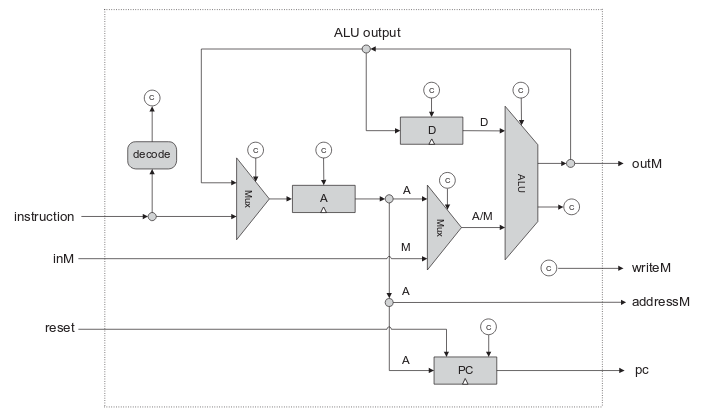
\includegraphics[scale=0.5]{pictures/cpu.png}
  \caption{CPU}
  \label{fig:cpu}
\end{figure}
\end{document}
